\documentclass[11pt]{scrartcl}
\usepackage[sexy]{evan}
\author{Konrad Kaczmarczyk}
\usepackage{amsmath,systeme}
\usepackage{listings}
\usepackage{graphicx}
\usepackage[T1]{fontenc}
\begin{document}
  \title{Analiza I.2*}
  \subtitle{Notatki z ćwiczeń}
 \maketitle
 \section{26 luty - pochodne}
     
  \begin{zadanie}
      Narysowano styczne do paraboli $y = x - \frac{1}{4} y^2$ w punktach $\left ( 0, 0 \right )$, $\left ( 2,1 \right )$ i $\left ( 4, 0 \right )$. Znajdź równania tych stycznuch bez stosowania pochodnych.
  \end{zadanie}
  
  \begin{walk}
      \item Dla $\left ( 2, 1 \right )$ wystarczy zauważyć że to wierzchołek, więc $y = 0$ spełnia.
      \item W pozostałych przypadkach wystarczy rozwiązać układy:
        \[
            \begin{cases}
                y = ax \\
                y = x - \frac{1}{4} x^2
            \end{cases}
            \qquad
            \begin{cases}
                y = a (x-4) \\
                y = (x-4) - \frac{1}{4} (x -4)^2
            \end{cases}
        \]
        które możemy rozwiąać z pomocą delty.
  \end{walk}
  \begin{zadanie}
      Pod jakim kątem przecinają się wykresy funkcji 
      \begin{enumerate}
          \item $ y = x^2 $ i $x = y^2$
          \item $y = \sqrt{\frac{1}{x}}$ i $y = \sqrt[3]{x}$ ?
      \end{enumerate}
  \end{zadanie}

  \begin{walk}
      \item Rozwiązujemy układ
        \[
            \begin{cases}
                x = y^2 \\
                y = x^2 \\
            \end{cases}
        \]
        otrzymujemy rozwiązania: $\left ( x, y \right ) \in \{\left ( 1,1 \right ), \left ( 0, 0 \right )\}$, przypadek drugi jest łatwy bo styczne do wierzchołków paraboli przecinają się pod kątem prostym.
        W pierwszym przypadku liczymy styczne, mianowicie: $x= 2y -1$, oraz $y= 2x -1$, licząc kąt między nimi otrzymujemy $\frac{\pi}{2} - 2 \text{arctg} \frac{1}{2}$
        
        \item 
  \end{walk}
  
  
  \begin{zadanie}
      Korzystając jedynie z definicji pochodnej oblicz $f'(p)$, przy czym $f(p)$ jest tak określonem, by $f$ była ciągła w punkcie $p$:
      \begin{enumerate}
          \item $f(x) = x(x - 1)$, $p = 1$,
          \item $f(x) = (x - 2) \lvert x+3 \rvert$, $p=2$,
          \item $f(x) = \left ( ln x \right ) \sqrt{1+ 3x^2}$, $p=1$.
      \end{enumerate}
  \end{zadanie}

  \begin{walk}
      \item 
      \item $f'(2), f(x) = (x-2) \abs{x + 3}$
        \[
          f'(p) = \lim_{h \to 0} \frac{F(p+ h) - F(p)}{h} = \lim_{h \to 0} \frac{5h + h^2}{h}
        \]
        
  \end{walk}
  
  \begin{zadanie}
    Niech $f(x) = \text{tg} \left ( x \cdot \text{cos} \left ( x^2 \right ) \text{sin} \left ( \frac{\pi}{4} + \text{ln} \left ( 1 + \frac{x}{2} \right ) \right )  \right ) $ dla $-1  < x < 1$. Zbadaj, czy funkcja $f$ ma pochodną w punkcie 0. Oblicz $f''(0)$, jeśli istnieje lub wykaż, że funkcja $f$ pochodnej w punkcje 0 nie ma.
  \end{zadanie}
  
   \begin{gather*}
     f'(0) = \lim_{h \to 0} \frac{\text{tg} \left ( h \cdot \text{cos} \left ( h^2  \right )  \right ) \text{sin} \left ( \frac{\pi}{4} + ln \left ( 1 + \frac{h}{2} \right ) \right ) - f(0)}{h} = \frac{\sqrt{2}}{2} \cdot \lim_{h \to 0} \frac{\text{tg} \left ( h \text{cos} \left ( h^2 \right )  \right ) }{h} = \frac{\sqrt{2}}{2}
   \end{gather*}
   \begin{zadanie}
       \[
         \frac{\left (  \prod_{i = 1}^{n} f_i(x) \right )' }{\prod_{i =1}^{n} f_i(x)} = \sum \frac{f'_i (x)}{f'_i(x)}
       \]
       
   \end{zadanie}
   
   Dowód jest poprzez indukcję.

   \begin{zadanie}
       $f: \mathbb{R} \to \mathbb{R} $ różniczkowalna.
       $f(0) = 0$, $f'(0) = 1$
       Czy $\exists_{\eps > 0}$, takie że $f$ jest s cisle rosnąca na $\left ( -\eps, \eps \right )$ ? 
            
   \end{zadanie}
   Wystarczy postawić funkcje 
   \[
     f(x) = \begin{cases}
              0, \qquad x = 0 \\
              x + \alpha x^2 \text{sin} \left ( \frac{1}{x} \right ) 
            \end{cases}
   \]
   zatem:
   \[
     f'(0) = \lim_{x \to 0} \frac{x + \alpha  x^2 \text{sin} \left ( \frac{1}{x} \right ) - 0 }{x} = 1 + \lim_{x \to 0 } x \alpha \cdot \text{sin} \left ( \frac{1}{x} \right ) = \frac{1}{\sqrt{1 + x^2}}
   \]
   i wyierając odpowiedni parametr $\alpha$ tworzymy kontrprzykład.

   \begin{zaddom}
       Rozważamy lustro w kształcie paraboli $x = y^{2}$. Niech $c \in \mathbb{R} $. Promień świetlny biegnie od punktu $\left ( \infty  ,c  \right )$ do punktu $(c_{2}, c)$, a następnie ulega odbiciu zgodnie z zasadą: „kąt padania jest równy kątowi odbicia”. Uzasadnij, że po odbiciu promień świetlny przejdzie przez punkt $\left ( \frac{1}{4},0 \right )$. (Jest to ognisko paraboli $x = y^{2}$.)
   \end{zaddom}
   
\begin{przykład}
    $(x^x)' = e^{x ln \left ( x \right )} = x^x (1 + ln \left ( x \right ))$
\end{przykład}

\begin{przykład}
  \begin{gather*}
    (ln \left ( x + \sqrt{1 + x^2} \right ))' \\
    = \left ( 1 + \sqrt{1 + x^2} \right )' \left ( ln \left ( y \right ) \right )' = \dots = 1
  \end{gather*}
\end{przykład}

\begin{zadanie}
    \[
      f(x) = \begin{cases}
        5x^2 + ax, \qquad x \leq 0 \\
        2x + b, \qquad x > 0
      \end{cases}
    \]
    Znajdź $a, b$ że $f$ jest różniczkowalna.

\end{zadanie}

Wystarczy rozpatrzyć tylko przypadek gdy $p  = 0$, gdyż pochodna jest tylko pojęciem lokalnym.

Różniczkowalna w $p = 0$, czyli ciągła, zatem po obliczeniach $b = 0$, a zgodnosc pochodnych wymusza $a = 2$.

\begin{zaddom}
    Oblicz $f'(x)$, dla 
    \[
        f(x) = log_x \left ( \text{sin} \left ( x \right )  \right ) \qquad x \in \left (  0, \pi \right ), x \not = 1
    \]
    
\end{zaddom}

  \subsection{Rozwizania zadań domowych}
    
    \begin{enumerate}
      \item Zadanie rozwiążemy geometrycznie \\
        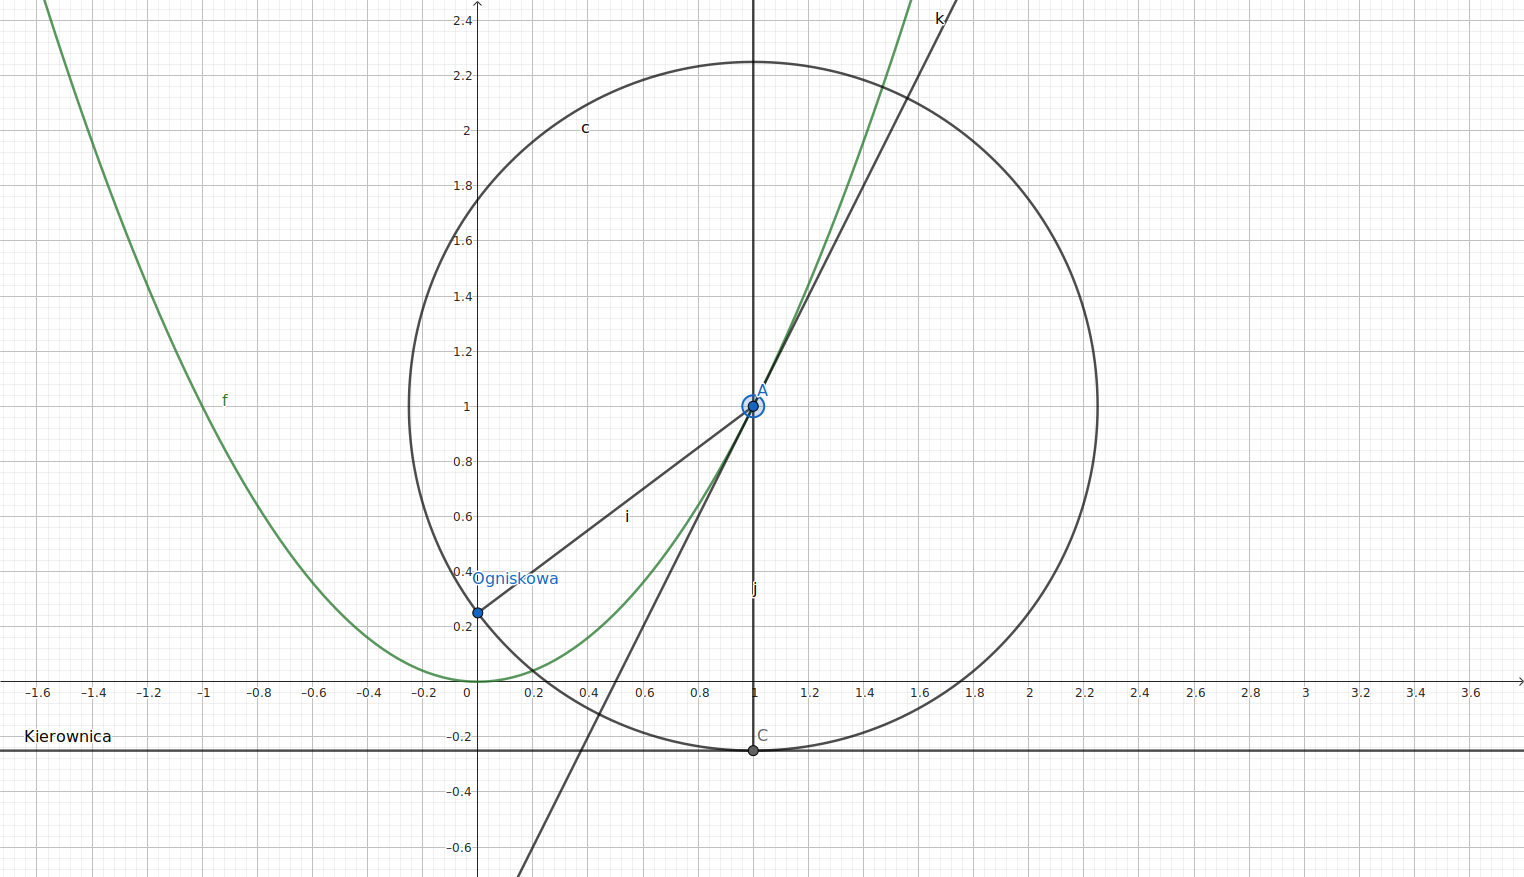
\includegraphics[width=\textwidth - 40pt]{parabola} \\
        Rozważmy geometrycznie czym jest styczna w punkcie $A$, mianowicie jest to prosta która przechodząca przez $A$, oraz punkt powstały poprzez przesunięcie się o infitezymalnie małą odległosć na paraboli. Zauważmy że trójkąt stworzony przez $A$, ognisko, oraz rzut prostopadły na kierownice, jest równoramienny, podobnie dla dowolnego punktu na paraboli, a także dla naszego infitezymalnie małego punktu. Wystarczy zauważyć zatem że jedyną opcją dla naszego punktu jest leżeć na wyskosci wypuszczonej z punktu $A$, więc jest styczną.

        Następnie zauważyć można kąty wierzchołkowe, oraz prawo odbicia (rysunek wyżej), i orzymujemy że wszystkie promienie po odbiciu przechodzą przez ognisko (czemu zawdzięcza swoją nazwę).

        Skończyć możemy zauważyć że punkt $\left ( 0, 0 \right )$, jest równo między ogniskiem a kierownicą, zatem znajdując rozwiązanie układu 
        \[
            \begin{cases}
                y = x^2 \\
                y = \frac{1}{2} x
            \end{cases}
        \]
        znajdujemy współrzędne punktu na paraboli który wraz z kierownicą i ogniskiem tworzy kwadrat zatem wpółrzędna $y$ tego punktu czyli $\frac{1}{4}$ jest współrzędną ogniska.
        
       \item Korzystając z wzorów na zmianę podstawy logarytmu i pochodną ilorazu otrzymujemy: 
         \begin{gather*}
           \left ( \text{log}_{x} \left ( \text{sin} \left ( x \right )  \right )  \right )^{'} = \left ( \frac{\text{ln} \left ( \text{sin} \left ( x \right )  \right ) }{\text{ln} \left ( x \right ) } \right )^{'} =
           \frac{\left ( \text{ln} \left ( \text{sin} \left ( x \right )  \right )  \right )^{'} \cdot \text{ln} \left ( x \right ) - \text{ln} \left ( \text{sin} \left ( x \right )  \right ) \cdot \frac{1}{x}}{\text{ln}^2 \left ( x \right ) } = \\ 
           \frac{\text{ctg}\left ( x \right ) \text{ln} \left ( x \right ) x - \text{ln} \left ( \text{sin} \left ( x \right )  \right )  }{x \text{ln}^2 \left ( x \right ) } 
         \end{gather*}
    \end{enumerate}
    \begin{zadanie}
        Niech $f : \left [ 0 ,1 \right ] \to \mathbb{R} $, $\left \{ 0 \right \} = 0$, $f'\left ( x \right ) > f \left ( x \right )$
    \end{zadanie}
    
    \subsection{Rozwązanie 1}
      Korzystamy z twierdznia o wartosci sredniej, i następnie z faktu o osiąg aniu swoich granic przez ciągłosc.
    \subsection{Rozwiązanie 2}
      Wystarczy zapisać że $f(x) = e^{x} g(x)$, z założeń otrzymujemy że $\left ( g \right )^{'} > 0$, i $g(0) = 0$, zatem funkcja jest rosnąca od $0$, co kończy dowód.
  \section{29 luty}
    \begin{przykład}
        \[
            f(x) =\text{arcsin} \left ( \frac{2x}{1+x^2} \right ) 
        \]
        Wyznacz styczną w punkcie $\left ( 1, f(1) \right )$.
    \end{przykład}
    
    Rozpatrzmy trójkąt o bokach: $2x$, $1+x^2$, i $1- x^2$. Przez $\alpha$ oznaczmy kąt naprzeciwko boku $2x$, zatem mamy:
    \begin{gather*}
        \text{tg} \left ( \alpha  \right ) = \frac{2x}{1 - x^2}, \qquad x = \text{tg} \left ( \beta  \right ) \\
        \text{tg} \left ( \alpha  \right )  = \text{tg} \left ( 2 \beta \right ) \Rightarrow \alpha = \beta \quad mod \pi  \\
        \alpha = 2 \text{arctg} \left (  x \right )  
    \end{gather*}

    \begin{zadanie}
        \begin{walk}
            \item Niech $f(x) = x^2 + x$, wyznacz styczną w punkcie $\left ( 1, 2 \right )$.
            \item Wykaż że istnieje funkcja odwrotna w przedziale $\left ( -\frac{1}{2}, + \infty  \right )$ ( $g = {f}^{-1} $)
            \item Pokaż że $g \left ( 2 \right ) = 1$, i oblicz $g'(2)$.
            \item Znajdź jawny wzór na $g$.
        \end{walk}
    \end{zadanie}
    
    \begin{walk}
        \item  $f'(1) = 2 \cdot 1 + 1 = 3$ , czyli $y = 3(x-1) + 2 \Rightarrow y = 3x - 1$.
        \item  W punkcie $x = \frac{1}{2}$, jest wierzchołek paraboli, zatem na przedziale $\left ( \frac{1}{2}, +\infty  \right )$ uzyskuje każdą wartosc tylko jeden raz, zatem istnieje funkcja odwrotna.
        \item Patrz następne
        \item Wystarczy rozwiązać równanie $g^2 + g = x$, z pomocą delty.
    \end{walk}
    
    \begin{zadanie}
        \[
            f(x) = x + e^{x} \qquad x \in \mathbb{R} 
        \]
        Wyznacz funkcje odwrotną i jej pochodną w punkcie $x = 1$.
    \end{zadanie}
    
    Zauważmy że $\left ( f \right )^{'} = e^{x} + 1> 0$, więc jest rosnąca $\Rightarrow $ funkcja jest różnowartosciowa. 
    \begin{gather*}
        g'(1) = \frac{1}{f'(x_{0})} = \frac{1}{f'(0)} = \frac{1}{e^{0} + 1} = \frac{1}{2}
    \end{gather*}
    
    \begin{zadanie}
        \[
          f = \text{atg} \left ( x \right ) + \text{atg} \left ( \frac{1-x}{1+x} \right ) 
        \]
      Pokaż że $f = \frac{\pi }{4}$
    \end{zadanie}
    
    Rozwiązanie 1

    Obliczyć pochodne

    \begin{gather*}
      f' = \frac{1}{1 + x^2} + \frac{1}{1 + \left ( \frac{1-x}{1 + x} \right )^2} \cdot \left ( \frac{1-x}{1+x} \right )' = \frac{1}{1 + x^2} = \dots
    \end{gather*}
    
    Rozwiązanie 2:
    
    Skorzystaj z wzoru na sumę $\text{atg} \left (  \right ) $.

    \begin{zaddom}
        Zbadaj funkcje;
        \[
            f(x) =
            \begin{cases}
              \text{atg} \left ( \frac{1}{\abs{x} } \right ) \qquad &x \not = 0 \\
              \frac{\pi }{2} \qquad &x = 0
            \end{cases}
        \]
    \end{zaddom}

    \begin{zaddom}
        Podać przykład funkcji $f: \mathbb{R}  \to \mathbb{R} $, i $a \in \mathbb{R} $, $x_n \to a$, $z_n \to a$ i $f'(a)$ istnieje
        \[
            \lim_{n \to \infty } \frac{f(z_n) - f(x_n)}{z_n - x_n} \not = f'(a)  
        \]
    \end{zaddom}

    \begin{zadanie}
      Zbadaj różniczkowalnosć funkcji:
      \[
          f(x) = 
          \begin{cases}
              \text{arc tg} \left ( \frac{1}{\abs{x} } \right ) \qquad x \not = 0 \\
              \frac{\pi }{2} \qquad x = 0
          \end{cases}
      \]
  \end{zadanie}
      
  Z zajęć wiemy że funkcja $\text{arc tg} \left (  \right ) $ jest różniczkowalna na całym $\mathbb{R}$, więc funkcja $f$ również jest różniczkowalna, gdy $x \not = 0$, zatem wystarczy sprawdzić, jej różniczkowalnosć w tym punkcie.
  \begin{lemat}
    \hspace{0.5cm}
    \begin{center}
      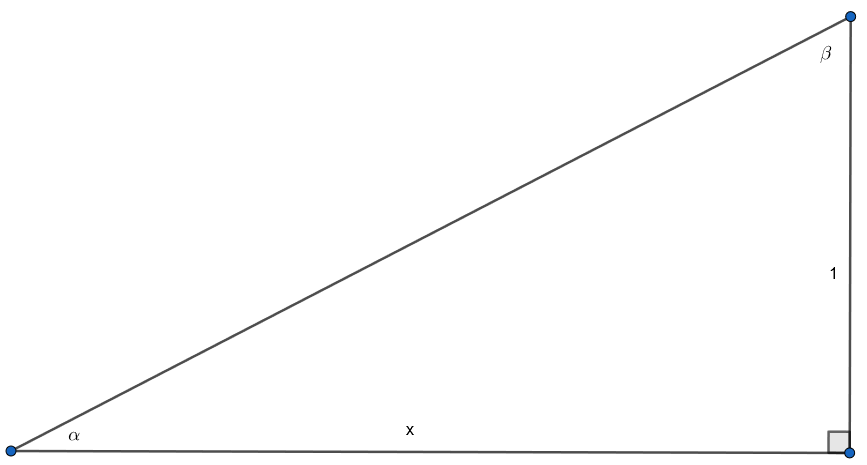
\includegraphics[width=12cm]{zaddom1}
    \end{center}
    Zauważmy że w trójkącie o bokach $x$, $1$, $\sqrt{x^2 + 1}$, występują następujące własnosci
    \[
        \begin{cases}
            \alpha + \beta = \frac{\pi }{2} \\
            \text{arc tg} \left ( \frac{1}{x} \right ) = \alpha \\
            \text{arc tg} \left ( x \right ) = \beta 
        \end{cases}
    \]
    Zatem zachodzi następujący lemat:
    \[
        \text{arc tg} \left ( \frac{1}{x} \right ) + \text{arc tg} \left ( x \right ) = \frac{\pi }{2}
    \]
  \end{lemat}
  
  Korzystając z lematu możemy obliczyć pochodne lewo i prawostronne:
  \begin{gather*}
      \lim_{x \to 0^+} \frac{\text{arc tg} \left ( \frac{1}{x} \right )  - \frac{\pi }{2}}{x} = \lim_{x \to 0^+} - \frac{\text{arc tg} \left ( x \right ) }{x} = -1 \\
      \lim_{x \to 0^-} \frac{\text{arc tg} \left ( \frac{1}{\abs{x}} \right ) - \frac{\pi }{2}}{x} = \lim_{x \to 0^-} - \frac{\text{arc tg} \left ( |x| \right ) }{x} = 1   
  \end{gather*}
  Gdzie po drodze skorzytalismy z granicy $\frac{\text{arc tg} \left ( x \right ) }{x} \to 1$, którą możemy otrzmyać z granicy $\frac{\text{tg} \left ( x_n \right ) }{x_n} \to 1$, dla $x_n \to 0$, i podstaiwając $x_n = \text{arc tg} \left ( b_n \right ) $, gdzie $b_n \to 0$.

  \begin{zadanie}
      Podaj przykład funkcji $f$, punktu $p$ i ciągów $\left ( x_n \right )$, $\left ( z_n \right )$ takich że $\lim_{n \to \infty } x_n  = \lim_{n \to \infty } z_n = p$, $z_n, x_n \not = p$, oraz funkcja $f$ jest równiczkowalna w punkcie $p$, ale
      \[
          \lim_{n \to \infty } \frac{f \left ( x_n \right ) - f \left ( z_n \right )}{x_n - z_n} \not = f'(p)
      \]
  \end{zadanie}
  
  Moim pomysłem jest skorzystanie z funkcji nie analitycznych, np:
  \[
      f(x) = 
      \begin{cases}
        x^2 + x \qquad x \in \mathbb{Q} \\
        x   \qquad x \not \in \QQ 
      \end{cases}
  \]
  Łatwo sprawdzić że, w punkcie $p = 0$, mamy pochodną równą zero bo $\abs{\frac{f(x) - f(0)}{x} -1}  = \abs{\frac{f(x)}{x} -1} $, które dla $x \not \in \QQ$: $\abs{\frac{x}{x} - 1} = 0$, i w pozostałych przypadkach $\abs{\frac{x^2 + x}{x} - 1} = \abs{x} \to 0$.

  Pozostało znaleźć odpowiednie $(x_n)$, i $(z_n)$. Wystarczające jest:
  \[
    x_n = \frac{1}{n} \qquad z_n = \frac{1}{n} + \frac{\pi}{n^3} 
  \]
  gdyż po obliczeniach mamy że:
  \[
    \lim_{n \to \infty } \frac{\frac{1}{n^2} + \frac{1}{n} - \frac{1}{n} - \frac{\pi }{n^3}}{\frac{1}{n} - \frac{1}{n} - \frac{\pi }{n^3}} =  \lim_{n \to \infty }  - \frac{n - \pi }{\pi } \not = 1   
  \]

  \section{5 marca}

  \begin{przykład}
      Wyznacz maksima funkcji
      \[
          \abs{x^2 - 2x - 3} + \frac{3}{2} \text{ln} \left ( x \right ) \qquad x \in \left [ \frac{1}{2}, 2 \right ]
      \]
  \end{przykład}
  
  \begin{lemat}
    Jesli $f$ jest minimalna na $\left ( x_{0} - \eps, x_{0} + \eps \right )$ i ma \ul{lokalne} ekstremum w $x_{0}$ to $f'(x_{0}) = 0$.
  \end{lemat}
  
  $f$ przyjmuje kresy tj. $\exists_{x_{1}, x_{2}} f(x_{1}) = \text{sup}_{x \in \left [ \frac{1}{2}, 2 \right ]} f $, $f(x_2) = \text{inf} \dots $.

  \[
      x^2 + 2x - 3 = 0 \Rightarrow x = -3, 1
  \]
  
  Rozważamy dwa przedziały $\left [ \frac{1}{2}, 1 \right ]$, i $\left [ 1, 2 \right ]$, i pochodne na tych przediałach:
  \[
      f' = 
      \begin{cases}
        2x + 2 + \frac{3}{2} \cdot \frac{1}{x} \qquad x &\geq 1 \\
        -2x + 2 + \frac{3}{2} \cdot \frac{1}{x} \qquad x &< 1
      \end{cases}
  \]

  \[
      4x^2 + 4x -3 = 0 \Rightarrow x = -\frac{3}{2}, \frac{1}{2} 
  \]
  
  \[
      4x^2 + 4x + 3 = 0 \Rightarrow \; \text{nie istnieje} 
  \]
  
  Po sprawdzeniu $\frac{1}{2}$ to minimum, a $2$ to maksimum

  \begin{przykład}
      Wyznacz ekstrema funkcji:
      \[
        f = 2 e x \text{ln} \left ( x \right ) \qquad x \in (0, 2]
      \]
  \end{przykład}
  
  \begin{gather*}
      f' = 2e \left ( \text{ln} \left ( x \right ) + 1 \right ) = 0 \iff  x = {e}^{-1} \\
      \lim_{x \to 0} x \text{ln} \left ( x \right ) = \lim_{y \to \infty } \frac{z}{e^z} \rvert_{x = e^{-z}} = 1   
  \end{gather*}

  \begin{zadanie}
    Wielomian $P(x)$ ma $n$ różnych pierwiastków $\Rightarrow $ P' ma conajmniej $n-1$ różnych pierwiastków.
      
  \end{zadanie}
  
  Korzystając z twierdzenia Rolle'a, wybieramy dwa kolejne pierwiastki, i otrzymujemy że między nimi istnieje pierwiastek $P'$, co kończy dowód.

  \begin{zadanie}
    Wiemy że $f : [a, \infty ) \to \mathbb{R} $, jest różniczkowalna i $\lim_{x \to +\infty } f'(x) = c $. Udowodnij że:
    \[
        \lim_{x \to + \infty } \left ( f(x+1) - f(x) \right ) = c  
    \]
    
  \end{zadanie}
  
  Skorzystać z tw. Lagrange'a

  \begin{zadanie}
      \[
          f = x^2, \quad g = x^3 \qquad x \in \left [ -1, 1 \right ]
      \]
      Czy istnieje takie $\eps \in \left ( -1,1 \right )$ takie:
      \[
          \frac{f(1) - f(-1)}{g(1) - g(-1)} = \frac{f'(\eps)}{g'(\eps)}
      \]
     Które założenie tw. Cauchy'ego nie jest spełnione?
  \end{zadanie}

  1 Rozwiązanie:

  Geometrycznie możemy narysować krzywą

  \begin{center}
    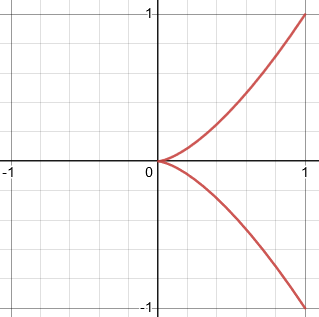
\includegraphics{krzywa}
  \end{center}
  
  i zauważyć że wektor prędkosci nigdy nie jest równoległy do odcinka (1,-1) - (1,1).

  2 Rozwiązanie:

  W tw. Cauchy'ego nie jest spełniony warunek $g' \not = 0$, i podstawić wartosci.

  \begin{zadanie}
    Niech $f,g,h : \left [ a, b \right ] \to \mathbb{R} $ będą funkcjami ciągłymi, różniczkowalnymi na $(a, b)$. Niech:
    \[
      F(x) = \text{det}
        \begin{bmatrix}
          f(x) & g(x) & h(x)  \\
          f(a) & g(a)  & h(a)   \\
          f(b) & g(b) & h(b) 
        \end{bmatrix}
    \]
    Udowodnij, że istnieje $x_{0} \in (a, b)$ takie, że $F'(x_{0}) = 0$. Wywnioskuj stąd twierdzenia Cauchy’ego i Lagrange’a o wartości średniej.
  \end{zadanie}
  
  Wiemy że $F(a) = F(b) = 0$, i korzystając z tw. Rolle'a mamy tezę.
  \begin{enumerate}
      \item stosując $F'(x)$, z $h = 1$, otrzymujemy tw. Cauchy'ego
        \[
            \frac{f'(x)}{g'(x)} = \frac{f(a) - f(b)}{g(a) - g(b)}
        \]
        
      \item  
  \end{enumerate}

  \begin{zadanie}
      Tak jak poprzednio niech $f$ będzie ciągłe i różniczkowalne na $\left [ a, b \right ]$, wykaż że:
      $\text{f nie jest liniowa} \Rightarrow \exists_{x_{1}, x_{2} \in (a,b)} $
      \[
          f'(x_{1}) < \frac{f(b) - f(a)}{b - a} < f'(x_{2})
      \]
      
  \end{zadanie}

  \begin{gather*}
  \exists_{x_{0} \in (a,b)} f'(x_{0}) = \frac{f(b) - f(a)}{b -a} \\
  F(x) = f(x) - x \cdot \frac{f(b) - f(a)}{b-a} \\
  F' = f' - \frac{f(b) - f(a)}{b - a} \\
  F'(x_{0}) = 0 \\ 
  \vdots
  \end{gather*}
  
  Niech $l(x)$ będzie funkcją linową z $\left ( a, f(a) \right )$ do $\left ( b, f(b) \right )$.
  \[
    \exists{x_{0}} f(x_{0}) > l(x_{0})
  \]
  
  Zatem z tw. lagrange'a mamy
  \[
      f'(x_{2}) = \frac{f(x_{0}) - f(a)}{x_{0} -a} > \frac{f(b) - f(a)}{b - a} > \frac{f(b) - f(x_{0})}{b - x_{0}} = f'(x_{1})
  \]
  
  \begin{zaddom}
     \[
       f = 4x +  \frac{9 \pi^2}{x} + \text{sin} \left ( x \right ) \qquad x \in \left [ - \pi , 2 \pi  \right ]
    \]
    Znajdź maksima i minima funkcji $f$.
  \end{zaddom}
    Korzystając z lematu Fermata, wiemy że funkcja swoje ekstrema gdy $f' = 0$, zatem obliczmy:
    \[
      f' = 4 - \frac{9\pi^2 }{x^2} + \text{cos} \left ( x \right )
    \]
    Przeanalizujmy osobno funkcje $4 - \frac{9 \pi^2}{x^2}$, i $\text{cos} \left ( x \right ) $.
    \begin{enumerate}
        \item dla $4 - \frac{9\pi^2}{x^2}$ wiemy że w punkcie $x = \frac{3}{2} \pi $ punkt zerowy, dla $x < \frac{3}{2} \pi $, jest ujemna, a dla $x > \frac{3}{2} \pi $, jest dodatnia.
        \item dla $\text{cos} \left ( x \right ) $ mamy podobnie w punkcie $x = \frac{3}{2} \pi $ punkt zerowy, dla $x < \frac{3}{2} \pi $, jest ujemna, a dla $x > \frac{3}{2} \pi $, jest dodatnia. 
    \end{enumerate}
    
    Wiemy że suma dwóch funkcji dodatnich jest dodatnia, a ujemnych ujemna. Zatem w przedziale $\left [ \pi , 2\pi  \right ]$, występuje jedno miejsce zerowe pochodnej. Po podstawieniu kolejno, $x = \pi, \frac{3}{2} \pi , 2\pi  $, znajdujemy ekstrema mianowicie 

    \[
      \min_{x \in \left [ \pi , 2\pi  \right ]} f(x) = 12 \pi  - 1 \qquad \max_{x \in \left [ \pi , 2\pi  \right ]} f(x) = 13 \pi  
    \]

    \begin{zaddom}
          Niech  $f(x)=x^2$, jeśli   $0<x<2$, i $x$ jest liczbą wymierną, $f(x)=2x-1$ jeśli $0<x<2$, ale $x$ jest liczb niewymierną i $f(x)=2x-4$  jeśli $x \in (2,3)$ jest taką liczbą wymierną, że $ \sqrt{2x - 4} $ jest liczba niewymierną. Wykazać, że funkcja $f$ jest różniczkowalna w $x_{0}=1$, $f'(1) \not = 0$, ma funkcję odwrotną, ale funkcja odwrotna nie jest różniczkowalna w punkcie $y0=f(1)=1$.
    \end{zaddom}
    
     \begin{center}
         \begin{asy}
           size(14cm, 3cm, IgnoreAspect);
             import graph; 
Label f; 
f.p=fontsize(6); 
xaxis(-0.1,3.1,Ticks(f, 1.0)); 
yaxis(-1,4,Ticks(f, 1.0)); 
real f1(real x) 
{ 
return x^2; 
} 
real f2(real x)
{
  return 2*x -1;
}
real g1(real x)
{
  return 2*x - 4;
}
real g2(real x)
{
  return sqrt(2*x -4);
}
draw(graph(f1,0,2),dashdotted  + green);
draw(graph(f2,0,2),dashed + red);
draw(graph(g1,2,3),dashdotted + blue);
        \end{asy} 
     \end{center}
      
     Łatwo pokazać że:
     \begin{gather*}
         \lim_{h \to 0} \frac{f(1+h) - f(1)}{h} \leq \max \left ( 2, \lim_{h \to 0} \frac{2h + h^2}{h}  \right ) = 2 \\
         \lim_{h \to 0} \frac{f(1+h) - f(1)}{h} \geq \min \left ( 2, \lim_{h \to 0} \frac{2h + h^2}{h}  \right ) = 2
    \end{gather*}

    Zatem wiemy że $f'(1) = 2$, a także funkcja $f$ posiada funkcje odwrotną o definicji:
    \[
      {f}^{-1}(x) =  
        \begin{cases}
          \frac{1}{2} x + \frac{1}{2} \qquad  & x \not \in \QQ \\
          \sqrt{x} & x = a^2, a \in \QQ \\
          \frac{1}{2} x + 2 & x = a^2 , a \not \in \QQ
        \end{cases}
    \]

  I łatwo zauważyć że ta funkcja przy $x \to 1$, nie będzie równa $\frac{1}{2}$, gdyż dla ciągu $x_n = \frac{1}{p_n} \to 0$, definicja:
  \[
      \lim_{n \to \infty } \frac{\frac{1}{2} \frac{1}{p_n} + 2 - 1}{\frac{1}{p_n}} = \lim_{n \to \infty } \left ( \frac{1}{2} + p_n \right ) = \infty  
  \]
  Więc nie spełnia warunków.

  \section{7 marca}

  \begin{przykład}
      Wykaż że funkcją spełniającą
      \[
          f'' = -f
      \]
      są funkcje w postaci $f = a \text{sin} \left ( x \right ) + b \text{cos} \left ( x \right ) $.
  \end{przykład}
      Oznaczmy funkcje $\alpha $, i $\beta $
      \begin{gather*}
          \alpha \left ( x \right ) = f(x) \text{cos} \left ( x \right ) - f'(x) \text{sin} \left ( x \right ) \\
          \alpha' (x) = f' \text{cos} \left ( x \right ) + f \text{sin} \left ( x \right ) - f'\text{cos} \left ( x \right ) - f \text{sin} \left ( x \right ) = 0
          \beta \left ( x \right ) = f(x) \text{sin} \left ( x \right ) + f' \text{cos} \left ( x \right ) \\
          \beta' (x) = 0 \\
          \begin{bmatrix}
              \text{cos} \left ( x \right )  &  - \text{sin} \left ( x \right )  \\
              \text{sin} \left ( x \right )  & \text{cos} \left ( x \right )  \\
          \end{bmatrix}
          \cdot
          \begin{bmatrix}
              f \\
              f'  \\
          \end{bmatrix}
          =
          \begin{bmatrix}
               a \\
               b  \\
          \end{bmatrix}
      \end{gather*}
      Odwracając macierz obrotu otrzymujemy tezę.
      \begin{przykład}
          Wykaż że
          \[
            \text{arc tgh } \left ( x \right ) = \frac{1}{2} \text{ln} \left ( \frac{1+x}{1 - x} \right )  
          \]
          
      \end{przykład}
      Mając definicje $\text{sinh} \left ( x \right )  = \frac{e^x - e^{-x}}{2}$, i $\text{cosh} \left ( x \right )  = \frac{e^x + e^{-x}}{2}$, mamy że 
      \[
        \text{tgh} \left ( x \right ) = \frac{e^x - e^{-x}}{e^x + e^{-x}} = \frac{e^{2x} - 1}{e^{2x} + 1} 
      \]
      Biorąc funkcje odwrotną otrzymujemy tezę.

      Drugi sposób:

      Skorzystajmy z wzorów:
      \[
          \text{sinh}' x = \text{cosh}' x \qquad \text{cosh}' x = \text{sinh}' x   
      \]
     
      Licząc pochodną $\text{tgh} \left ( x \right ) $:
      \[
          \left ( \text{tgh } x \right )^{'} = \left ( \frac{\text{sinh} x }{\text{cosh} x } \right )^{'} = \dots = \frac{1}{\text{cosh}^2 x } = 1 - \text{tgh}^2  \left ( x \right ) 
      \]
      Więc 
      \[
        (\text{arc tgh} \left ( x \right ))' = \frac{1}{ \text{arc tg}' \left ( x \right ) } = \frac{1}{1 - \text{tgh}^2 \left ( x \right ) } = \frac{1}{1- y^2} 
      \]
      
      \begin{zadanie}
           $f,g : \left [ 0,1 \right ] \to \mathbb{R}$, ciągłe , różniczkowalne i niech $f(0) = f(1) = 0$, udowodnij że równanie ma rozwiązanie
           \[
               g' f + f' = 0
           \]
      \end{zadanie}
      Wystarczy podstawić $h : = e^g f$, i sprawdzić założenia.

      \begin{zadanie}
        $f : \left [ a,b \right ]  \to \mathbb{R} $ która jest różniczkowalna i ciągła, i niech $b - a > \pi $.
        Wykaż że
        \[
            f' < 1 + f^2
        \]
        ma rozwiązanie
      \end{zadanie}
      
      Podstawiając $g = \text{arc tg} \left ( f \right ) $, teza zmienia się w $\exists_{x_{0}} g'(x_{0}) < 1$,
      więc przez sprzecznosć w $g' \geq 1$, ale:
      \[
          \frac{g(b) - g(a)}{b -a} = g'(\eps) \geq 1 \Rightarrow g(b) - g(a) \geq \pi 
      \]
      co jest sprzeczne z zbiorem wartosci funkcji $\text{arc tg} \left ( x \right ) $, co kończy dowód.

      \begin{zadanie}
          $f: \mathbb{R}  \to \mathbb{R} $ jest dwukrotnie różniczkowalna i $f(a) = a$ dla $a = 0, 1, 2$, wykaż że istnieje takie $x_{0}$ takie że $f''(x_{0}) = 0$
      \end{zadanie}
      Połóżmy $h(x) = f(x) - x$, i korzystając dwukrotnie z twierdzenia Rolle'a otrzymujemy tezę.

      \begin{zadanie}
          Niech $f(x) = \sqrt[5]{\frac{(x+1)^2 (x-1)^6}{x}}$ zbadaj przebieg zmiennosci funkcji. 
      \end{zadanie}

      \begin{center}
      \begin{asy}
           size(8cm, 8cm, IgnoreAspect);
             import graph; 
Label f; 
f.p=fontsize(6); 
xaxis(0,8.1,Ticks(f, 1.0)); 
yaxis(0,8,Ticks(f, 1.0)); 
real f1(real x) 
{ 
return ((x+1)^2 * (x-1)^6 /x)^(1/6); 
} 
draw(graph(f1,0.1, 6));
        \end{asy} 
     \end{center}

     \section{12 marca}
         \begin{zadanie}
           Niech $f$ będzie funkcją różniczkowalną na $[a,b]$, $f'$ ciągła na $[a,b]$ i
             \[
                 f(a) = f \left ( b \right ) = f'\left ( a \right ) = f' \left ( b \right ) = 0
             \]
         \end{zadanie}

         Z tw. Rolle'a wiemy że istnieje takie $c$ że $f'(c) = 0$, i korzystając dwa kolejne razy otrzymujemy tezę.
         \begin{lemat}
           Niech $f,g: [a,b] \to \mathbb{R} $ ciągłe i różniczkowalne na przedziale $(a,b)$

           Jesli $f(a) = g(a)$, i $f' \leq g'$, wtedy $f(b) \leq g \left ( b \right )$, i odwrotnie.
         \end{lemat}
         
         \begin{przykład}
             \[
               \text{cos} \left ( x \right ) > 1 - \frac{1}{2} x^2
             \]
         \end{przykład}
         Co wynkika z nierównosci $\text{sin} \left ( x \right ) < x$.

         \begin{zadanie}
             \[
                 \text{ln} \left ( 1 + x^2 \right ) 
             \]
             sprawdź czy jest jednostajnie ciągła
         \end{zadanie}
         
         Wytarczy sprawdzić że $f' = \frac{2x}{1 + x^2}$, które jest ograniczone przez 1, zatem jest j.ciągłą.

         \begin{przykład}
             \[
                 f = \text{ln} \left ( 1 + x^x \right ) 
             \]
             czy jest j. ciągła
         \end{przykład}
         Wiemy że 
         \[
             f' = \frac{x^x (\text{ln} \left ( x \right ) + 1)}{1 + x^x} \to \infty
         \]
         Zatem 
         \[
             \text{sup} \left \{ f(x + \sigma) - f(x) : x \in D_f \right \} 
         \]
         Gdy przy $\sigma \to 0$, jest ograniczone, to funkcja jest j. ciągła.
         Ale przy ustalonej $\delta$ mamy:
         \[
             \frac{f(x + \delta) - f(x)}{\delta} = f'(\eps) \to + \infty 
         \]
         Więc nie jest j. ciągła.

         \begin{zadanie}
           Funkcja dana funkcja $f: [0, \pi - \text{arcsin} \left ( \frac{1}{\pi } \right ) ] \to \mathbb{R} $ jest wzorem
             \[
                 f = x \text{sin}^2 \left ( x \right ) + \text{sin} \left ( x \right ) \cdot \text{cos} \left ( x \right ) 
             \]
             Znajdź ekstrema tej funkcji.
         \end{zadanie}
         
      
\end{document}
